\documentclass[10pt]{beamer}

\usepackage[utf8]{inputenc}
\usepackage{float}
\usepackage[british]{babel}
\usepackage{amsmath, amsfonts, amssymb}
\usepackage{graphicx}
\usepackage{booktabs} 
\usepackage{tikz}
\usepackage{xcolor}

\usetheme{Madrid}
\usecolortheme{whale}
\setbeamertemplate{navigation symbols}{} 
\setbeamertemplate{headline}{}

\title[Processo Estocásticos II]{Trabalho Análise Espectral de Potência}
\author{Mateus Ribeiro Gomes}
\date{\today}

\begin{document}

\begin{frame}
    \titlepage
\end{frame}

% --- SEÇÃO 1: MODELAGEM ---
\section{Modelagem do Sistema}

\begin{frame}{Modelagem do Sistema: Sinais de Entrada}
    O sistema baseia-se na composição de três componentes principais:
    \vfill
    \begin{itemize}
        \item \textbf{Processo Autorregressivo AR(2):}
        \begin{equation*}
            x(n) = a_1 \cdot x(n-1) + a_2 \cdot x(n-2) + u(n)
        \end{equation*}
        Onde $a_1 = 1.35$, $a_2 = -0.85$ e $u(n) \sim \mathcal{N}(0, 1)$.
        
        \item \textbf{Canal FIR:}
        \begin{equation*}
            h(n) = \delta(n) + \alpha \cdot \delta (n-D)
        \end{equation*}
        Com ganho de atraso $\alpha = 0.72$ e atraso $D = 4$.
        \item \textbf{Interferência de Canal Adjacente:}
        \begin{equation*}
            s_{int}(n) = A \cdot \cos(2 \pi f_0 n + \phi)
        \end{equation*}
            Onde $f_0 = 0.45$ e $\phi \sim \mathcal{U}[0, 2\pi)$.
        
    \end{itemize}
\end{frame}

\begin{frame}{Modelagem do Sistema: Interferência e Saída}
    \begin{itemize}
        \item \textbf{Sinal Recebido Total:}
        \begin{equation*}
            r(n) = y(n) + s_{int}(n) + w(n)
        \end{equation*}
            Onde $w(n)$ é o Ruído Branco Gaussiano Aditivo (AWGN) com variância $\sigma_w^2$ ajustada conforme a SNR desejada, e $y(n)$ é o $x(n)$ após
            passar pelo canal FIR.
    \end{itemize}
\end{frame}

% --- TAREFA 1 ---
\section{Tarefa 1}
\begin{frame}{Tarefa 1: Sinal no Domínio do Tempo}
    \begin{itemize}
        \item Configuração: $A = \sqrt{2}$ (Potência unitária).
        \item Comparação entre janelas de $N = 1024$ e $N = 4096$.
    \end{itemize}
    \vfill
    \begin{figure}
        \centering
        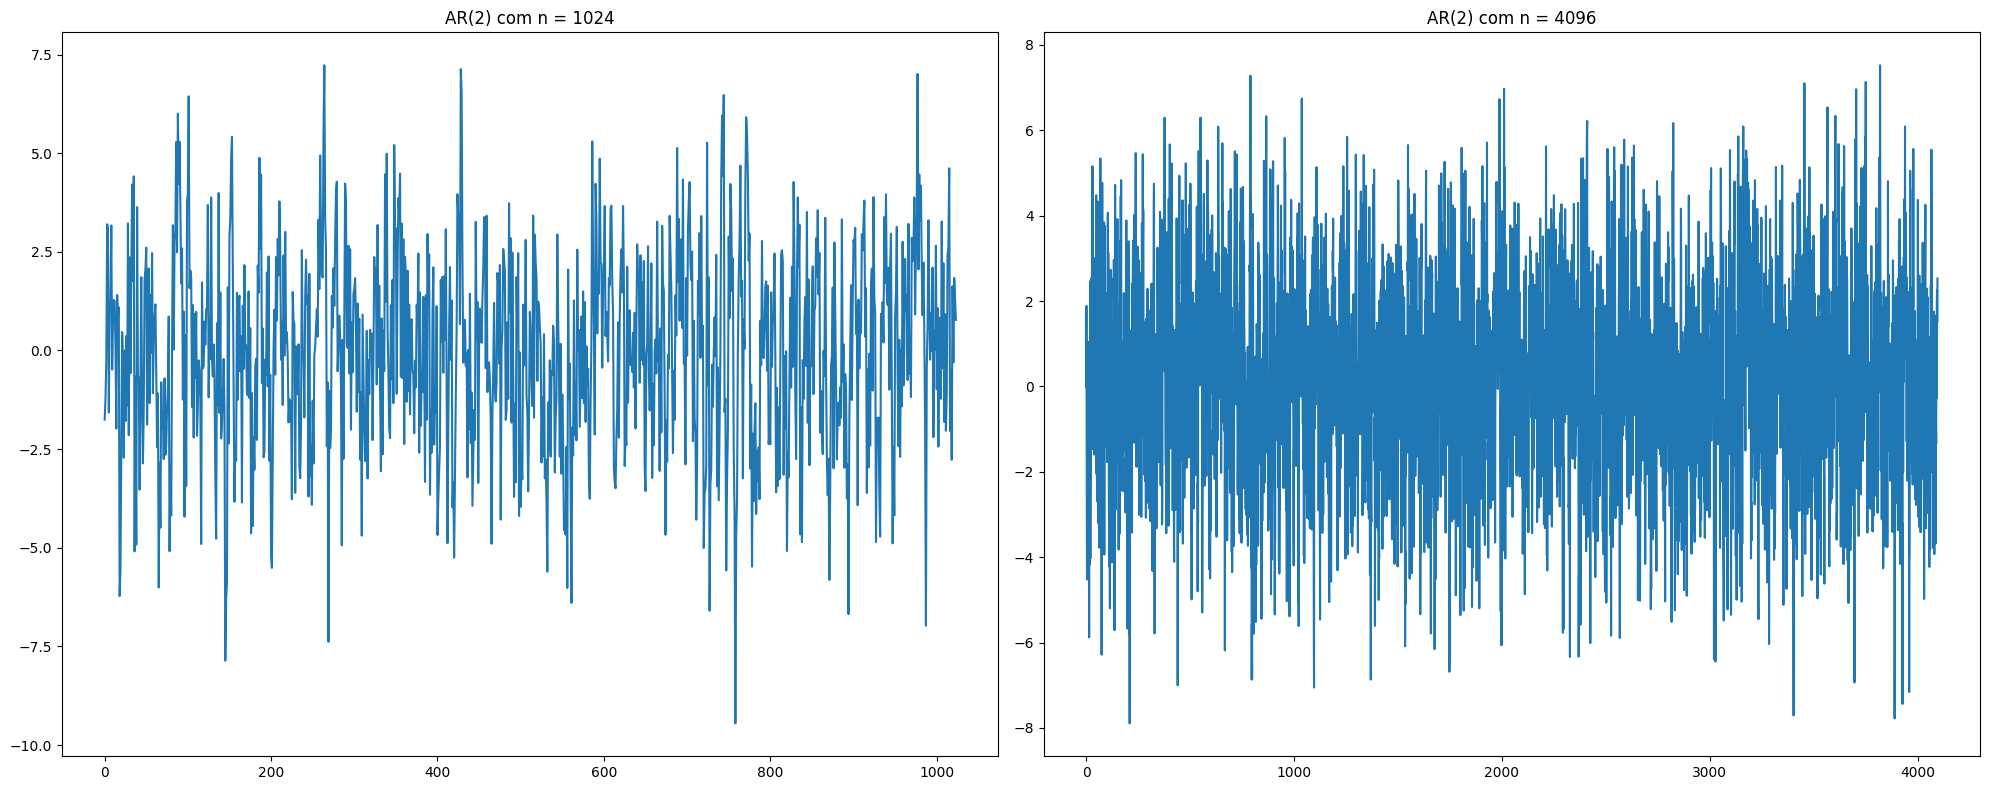
\includegraphics[width=0.8\textwidth]{tarefa1_tempo.png}
        \caption{Sinais $r(n)$ gerados para a Tarefa 1.}
    \end{figure}
\end{frame}

% --- TAREFA 2 ---
\section{Tarefa 2}
\begin{frame}{Tarefa 2: Parâmetros de Simulação e Cenários}
    Foram explorados 16 cenários combinando Amplitude ($A$) e SNR:
    \vfill
    \begin{columns}
        \begin{column}{0.5\textwidth}
            \textbf{Amplitudes (A):}
            \begin{itemize}
                \item $0.5$: Interferência fraca.
                \item $\sqrt{2}$: Equilíbrio energético.
                \item $5.0$: Interferência severa.
                \item $10.0$: Interferência extrema.
            \end{itemize}
        \end{column}
        \begin{column}{0.5\textwidth}
            \textbf{SNR (dB):}
            \begin{itemize}
                \item $0$ dB: Degradação máxima.
                \item $15$ dB: Condição nominal.
                \item $30$ dB: Alta qualidade.
                \item $50$ dB: Teórico ideal.
            \end{itemize}
        \end{column}
    \end{columns}
\end{frame}

\begin{frame}{Tarefa 2: Variância Ajustável ($\sigma_w^2$)}
    \centering
    \footnotesize
    \begin{tabular}{cccc}
        \toprule
        \textbf{N} & \textbf{A} & \textbf{SNR (dB)} & \textbf{Variância ($\sigma_w^2$)} \\
        \midrule
        1024 & 0.5 & 0 & 4.0455 \\
        1024 & 0.5 & 15 & 0.1272 \\
        1024 & $\sqrt{2}$ & 30 & 0.0038 \\
        1024 & 10.0 & 50 & 0.0000 \\
        4096 & 0.5 & 0 & 3.8300 \\
        4096 & $\sqrt{2}$ & 15 & 0.1370 \\
        4096 & 5.0 & 30 & 0.0040 \\
        4096 & 10.0 & 50 & 0.0000 \\
        \bottomrule
    \end{tabular}
    \vfill
    
    \begin{itemize}
        \item A variância é calculada com base na seguinte equação $$SNR_{db} = 10 \cdot log_{10} \cdot (\frac{P_{signal}}{P_{noise}})$$ 
            Queremos achar o $P_{noise}$, portanto $$P_{noise} = \frac{P_{signal}}{10^{\frac{SNR}{10}}}$$
    \end{itemize}
    \begin{itemize}
        \item Podemos ver que:
        \item $\sigma_w^2$ diminui com o aumento da SNR.
        \item O valor de $A$ causa flutuações pequenas, mas não altera a tendência da variância.
    \end{itemize}
\end{frame}

\begin{frame}{Tarefa 2: Matriz de Sinais no Tempo (N=1024)}
    \begin{figure}
        \centering
        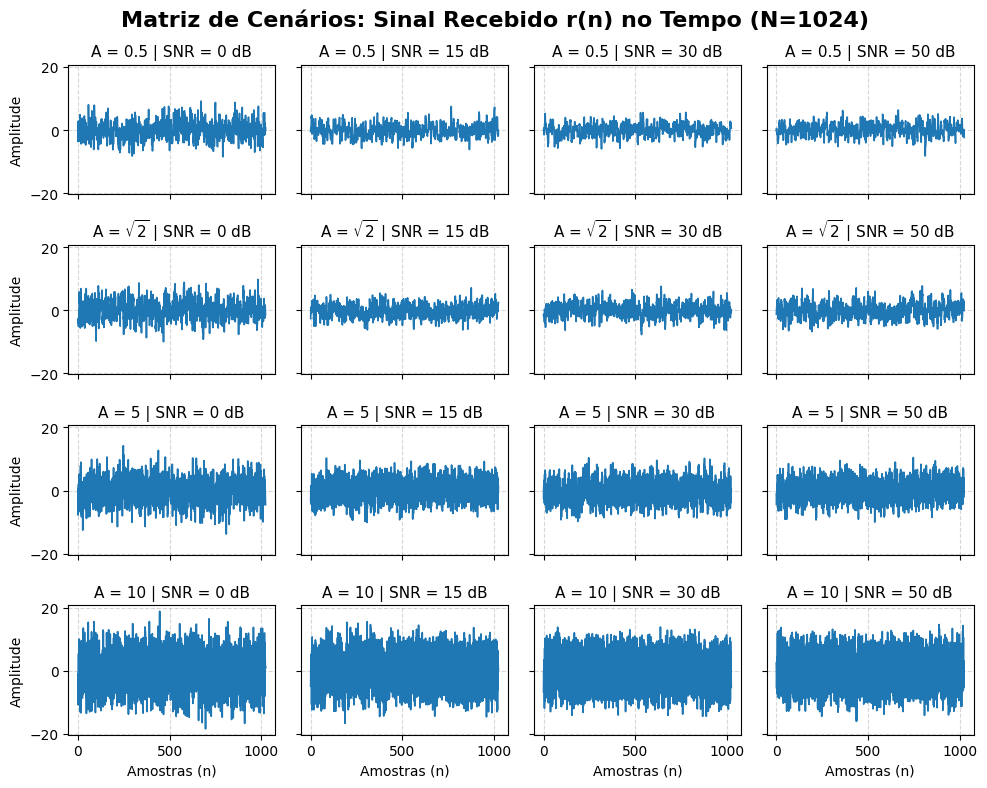
\includegraphics[width=0.8\textwidth]{tarefa2_n1024.png}
    \end{figure}
\end{frame}

\begin{frame}{Tarefa 2: Matriz de Sinais no Tempo (N=4096)}
    \begin{figure}
        \centering
        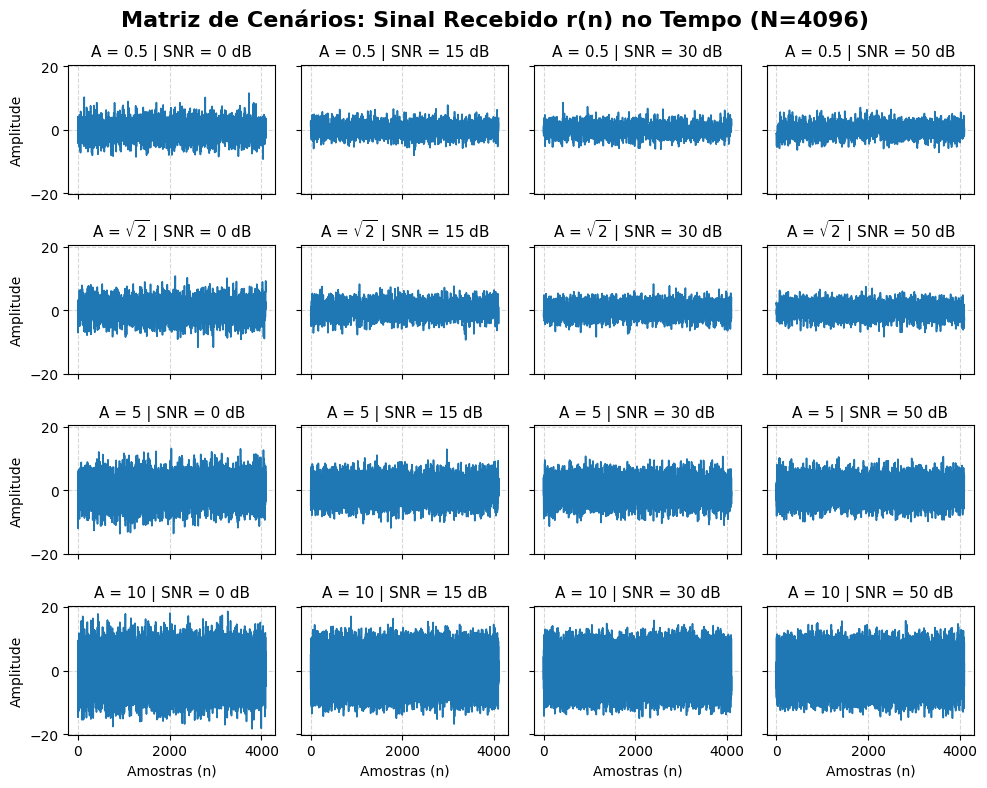
\includegraphics[width=0.8\textwidth]{tarefa2_n4096.png}
    \end{figure}
\end{frame}

% --- TAREFA 3 ---
\section{Tarefa 3}
\begin{frame}{Tarefa 3: Estimação Espectral (DEP)}
    Comparação entre dois métodos não-paramétricos:
    \vfill
    \begin{block}{1. Método do Periodograma}
        Baseado na DFT direta do sinal. Possui \textbf{máxima resolução}, porém é um estimador \textbf{inconsistente} (variância não converge para zero com o aumento de $N$).
    \end{block}
    \begin{block}{2. Método de Welch}
        Aplica médias de K periodogramas de segmentos. Reduz a variância ao custo da resolução espectral.

        Passo a passo do método:
        \begin{enumerate}
            \item O vetor original contendo a totalidade do sinal é subdividido
                em segmentos K menores de tamanho fixo.
            \item Calcula-se o periodograma individual de cada um dos K sub-blocos segmentados.
            \item O espectro final é obtido por meio da média de todos os periodogramas calculados na etapa anterior.
        \end{enumerate}
    \end{block}
\end{frame}

\begin{frame}{Tarefa 3: Periodogramas (N=1024)}
    \begin{figure}
        \centering
        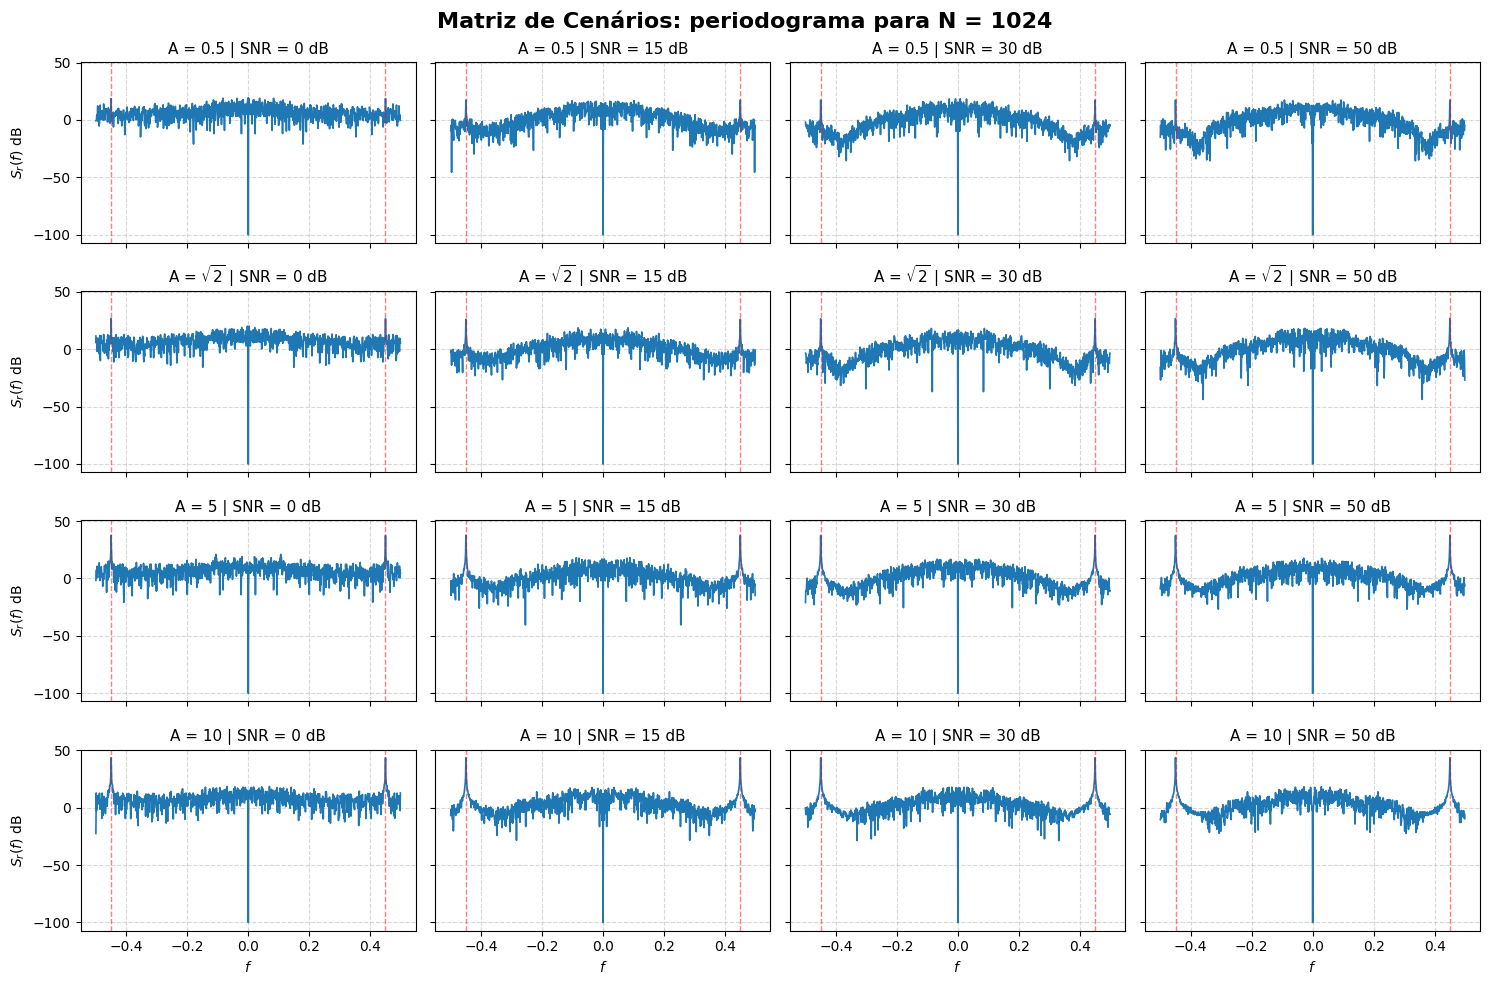
\includegraphics[width=0.9\textwidth]{period_1024.png}
    \end{figure}
\end{frame}

\begin{frame}{Tarefa 3: Periodogramas (N=4096)}
    \begin{figure}
        \centering
        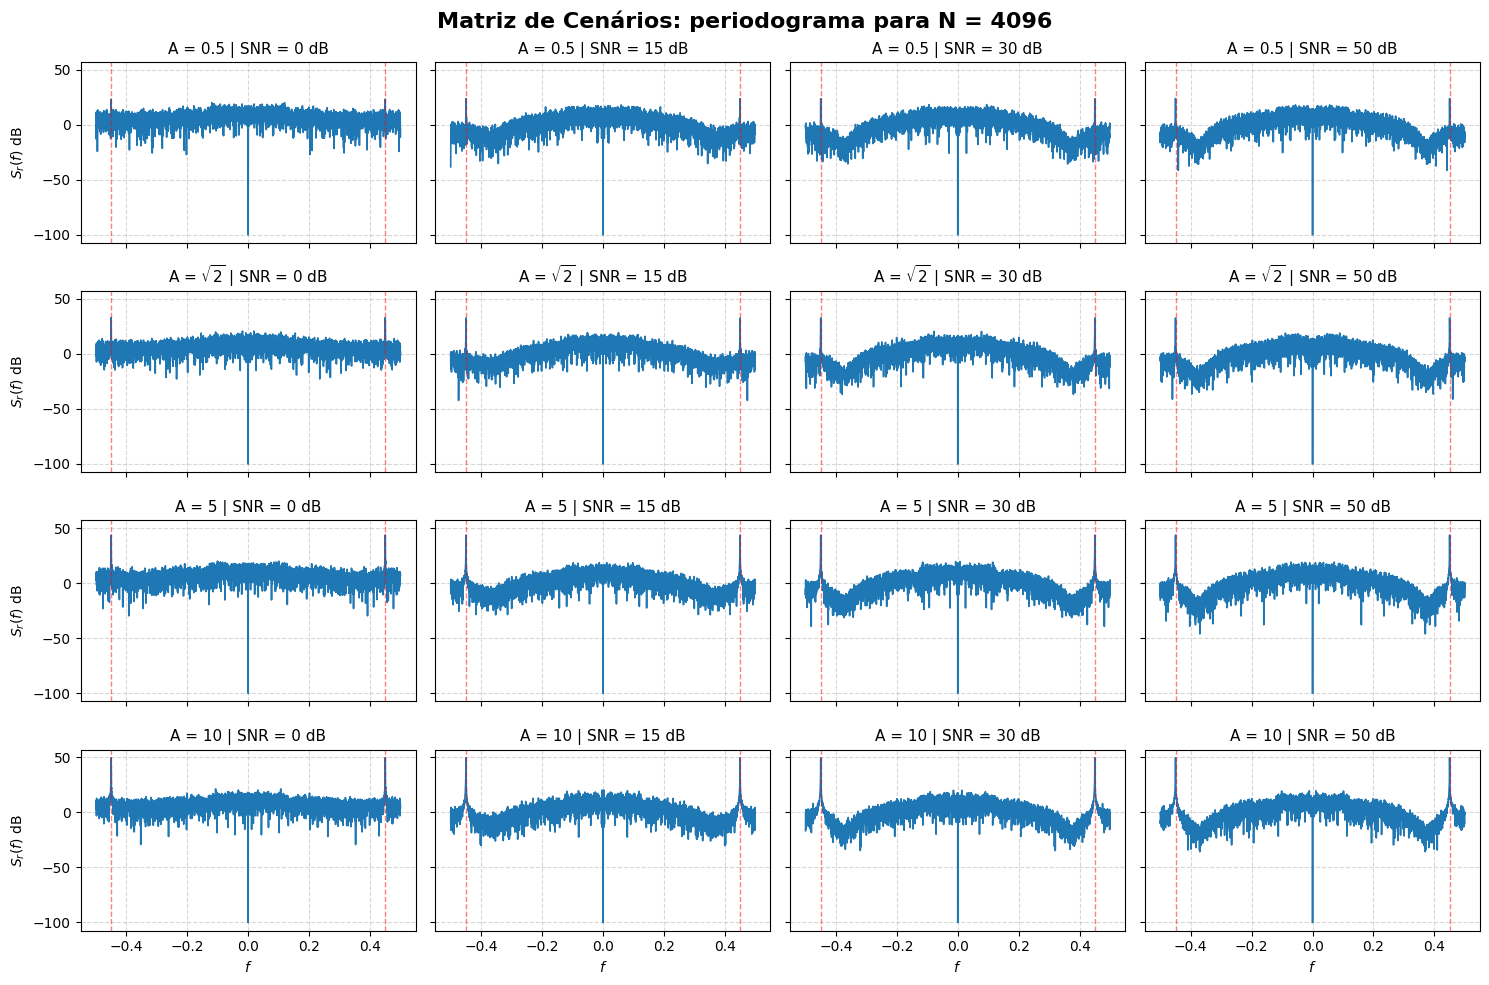
\includegraphics[width=0.9\textwidth]{period_4096.png}
    \end{figure}
\end{frame}

\begin{frame}{Tarefa 3: Método de Welch (N=1024)}
    \begin{figure}
        \centering
        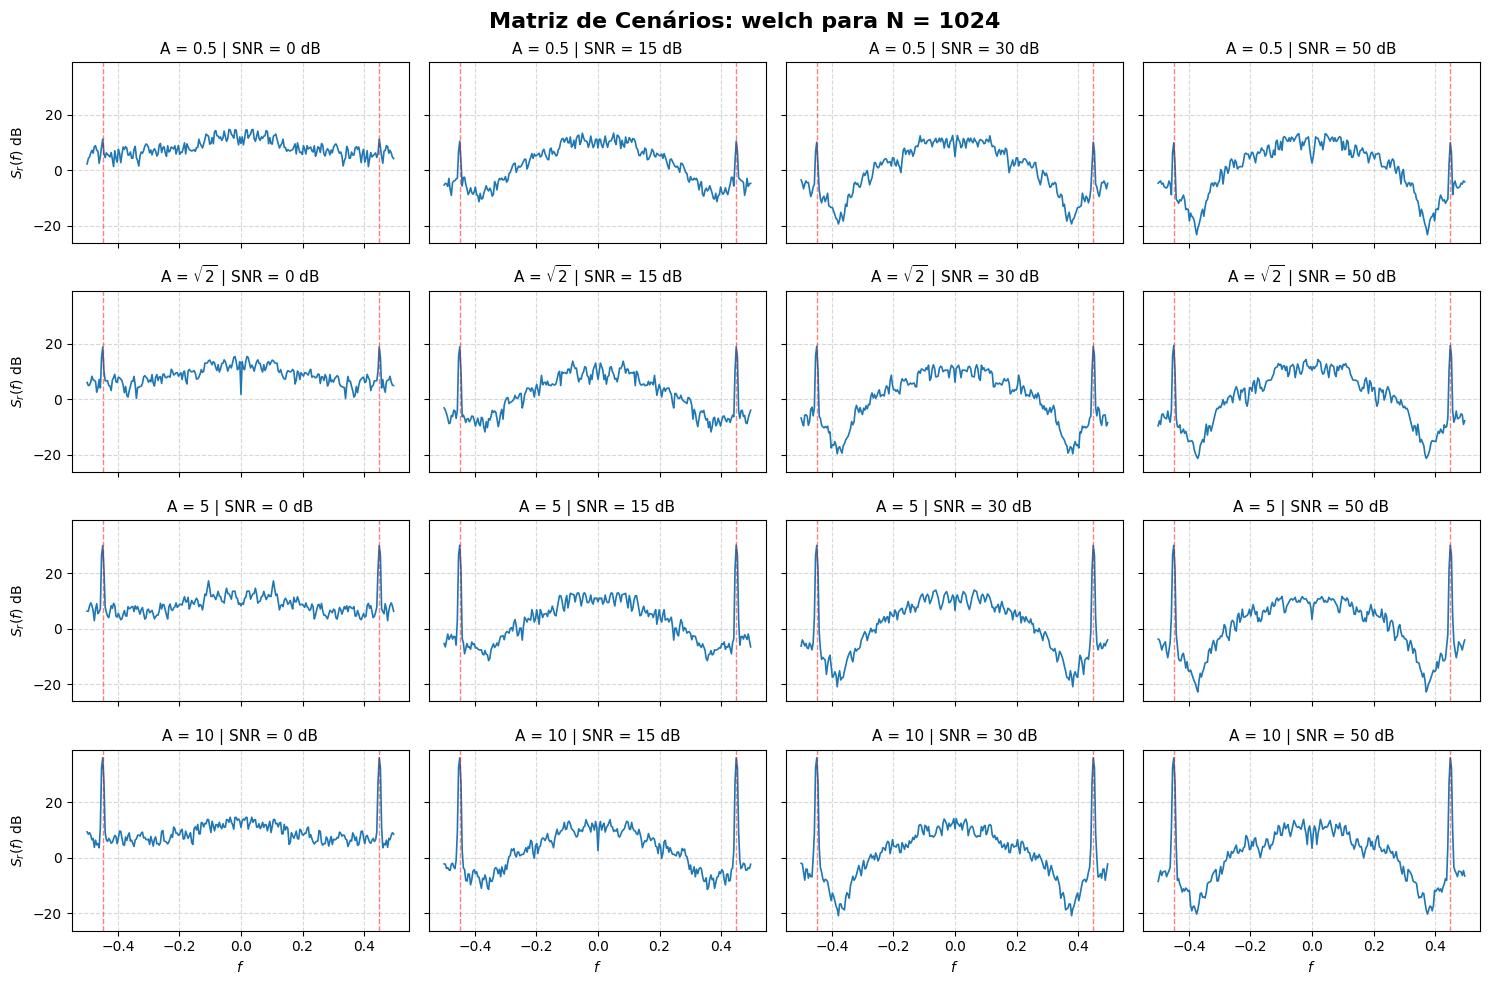
\includegraphics[width=0.9\textwidth]{welch_1024.png}
    \end{figure}
\end{frame}

\begin{frame}{Tarefa 3: Método de Welch (e N=4096)}
    \begin{figure}
        \centering
        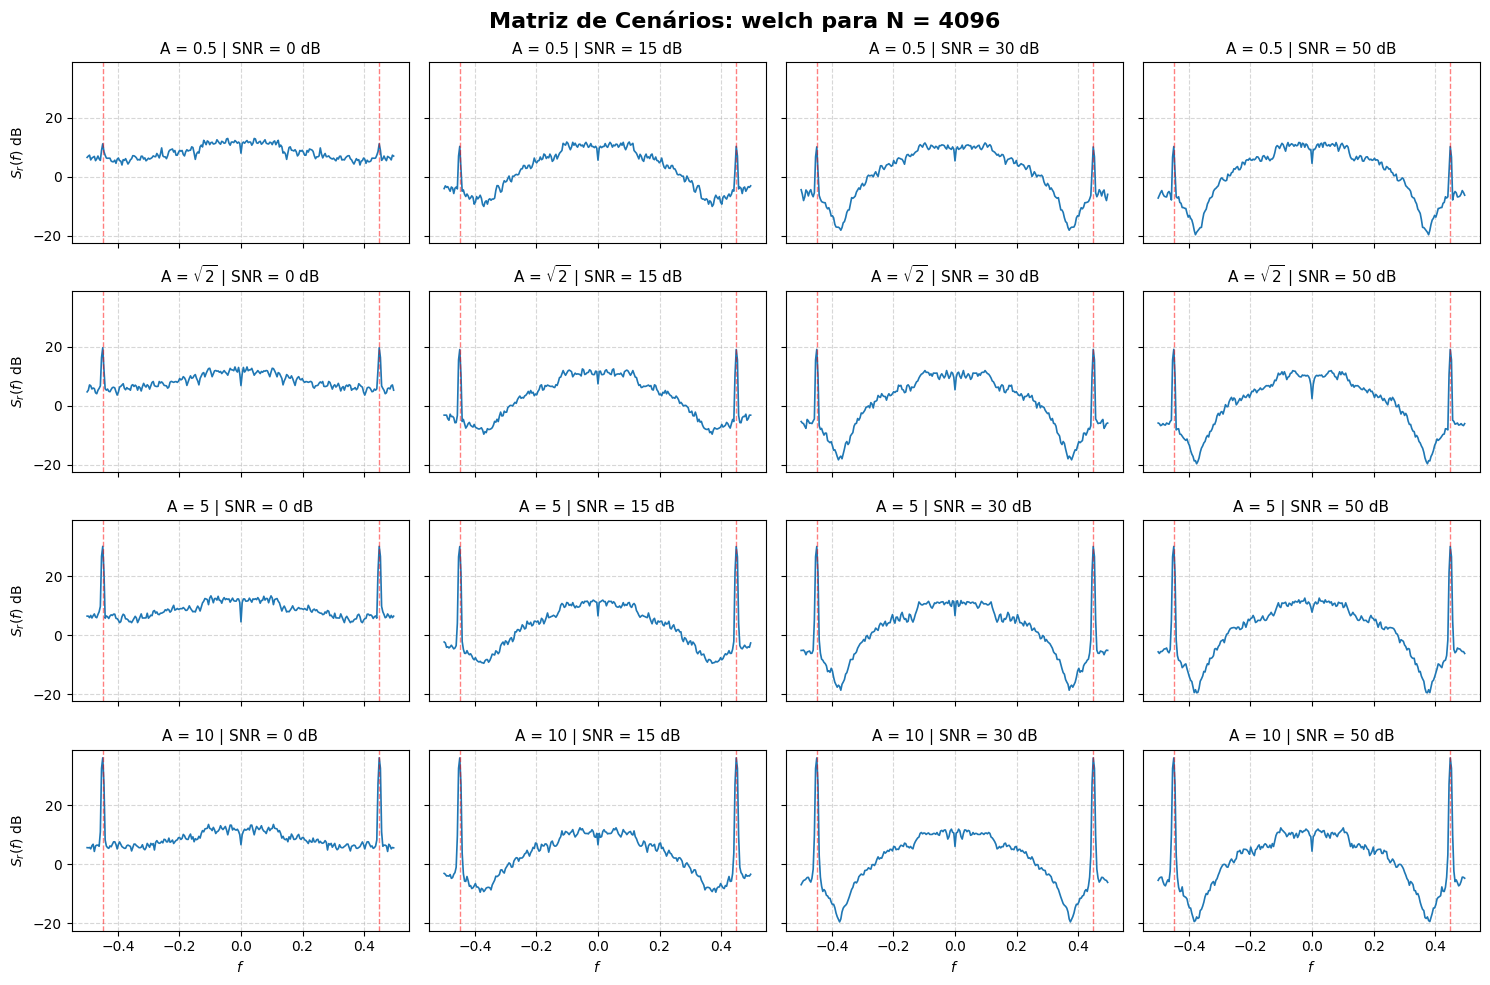
\includegraphics[width=0.9\textwidth]{welch_4096.png}
    \end{figure}
\end{frame}
% --- TAREFA 4 ---
\section{Tarefa 4}
\begin{frame}{Tarefa 4: Validação Teórica}
    A DEP teórica do sistema é modelada por:
    \begin{equation*}
        S_r(f) = |H(f)|^2 S_{xx}(f) + \frac{A^2}{4}[\delta(f-f_0) + \delta(f+f_0)] + \sigma_w^2
    \end{equation*}

    Onde:
    \begin{itemize}
        \item $H(f) = 1 + \alpha \cdot exp(-j2 \pi f D)$
        \item $S_x(f) = \frac{1}{|1 - a_1 \cdot exp (-j 2 \pi f) - a_2 \cdot exp(-j 4 \pi f)|^2}$
    \end{itemize}

    A comparação com as estimações foram feitas usando o \textbf{MSE}:
\end{frame}

\begin{frame}{Tarefa 4: Resultados de Validação Periodograma (N=1024)}
    \begin{figure}
        \centering
        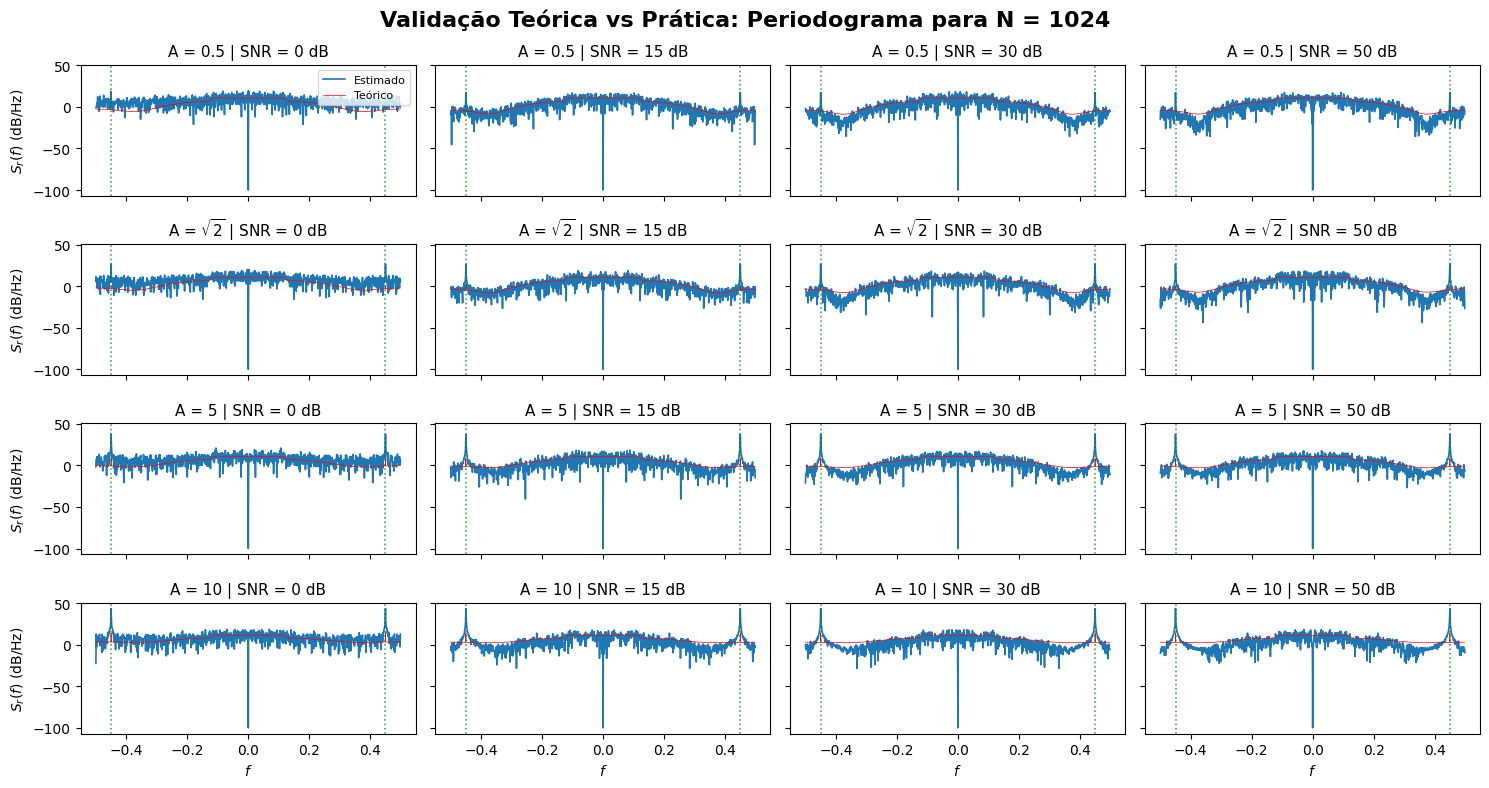
\includegraphics[width=0.9\textwidth]{valid_period_1024.png}
    \end{figure}
\end{frame}
\begin{frame}{Tarefa 4: Resultados de Validação Welch (N=1024)}
    \begin{figure}
        \centering
        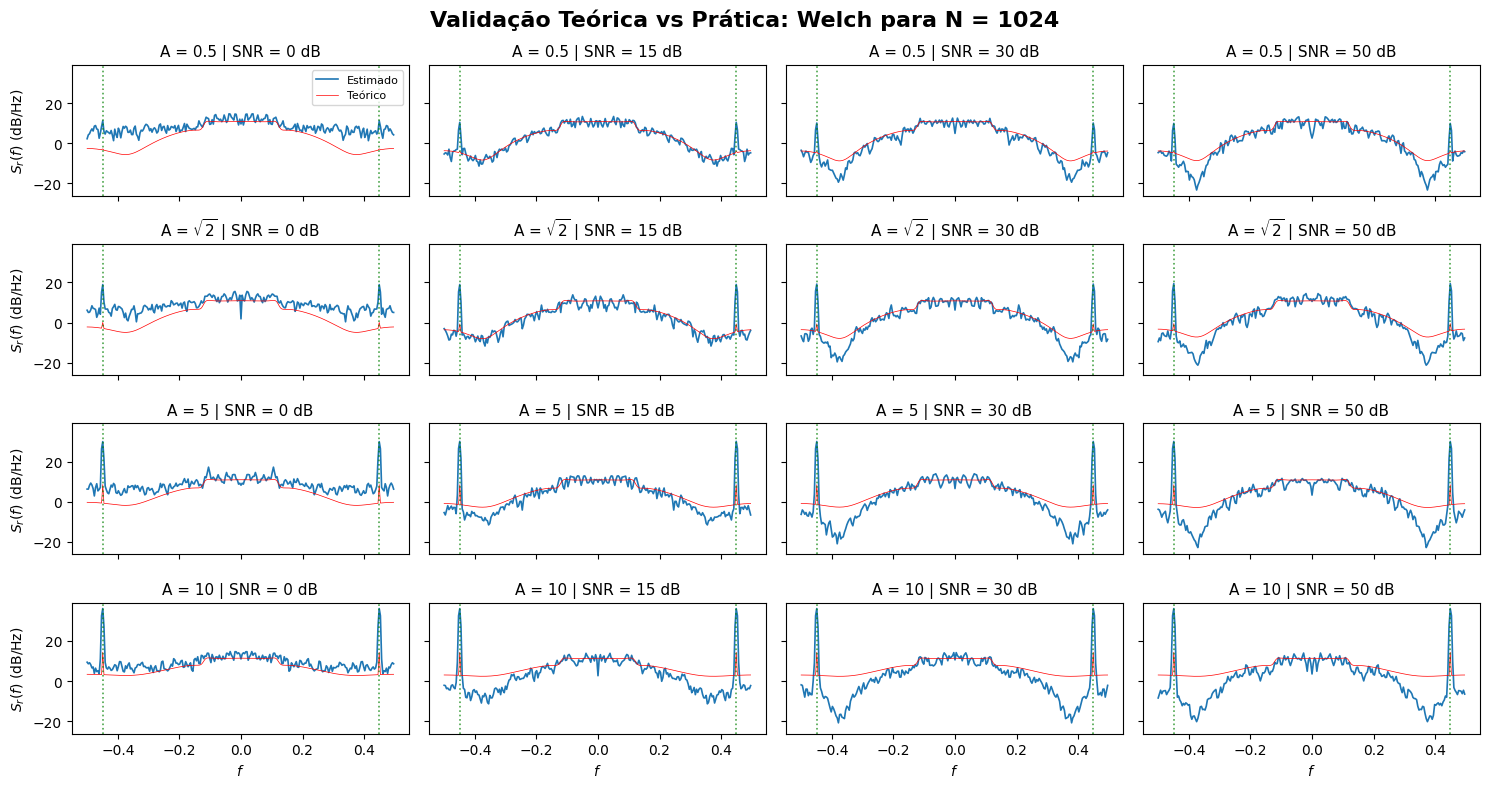
\includegraphics[width=0.9\textwidth]{valid_welch_1024.png}
    \end{figure}
\end{frame}

\begin{frame}{Tarefa 4: Resultados de Validação Periodograma (N=4096)}
    \begin{figure}
        \centering
        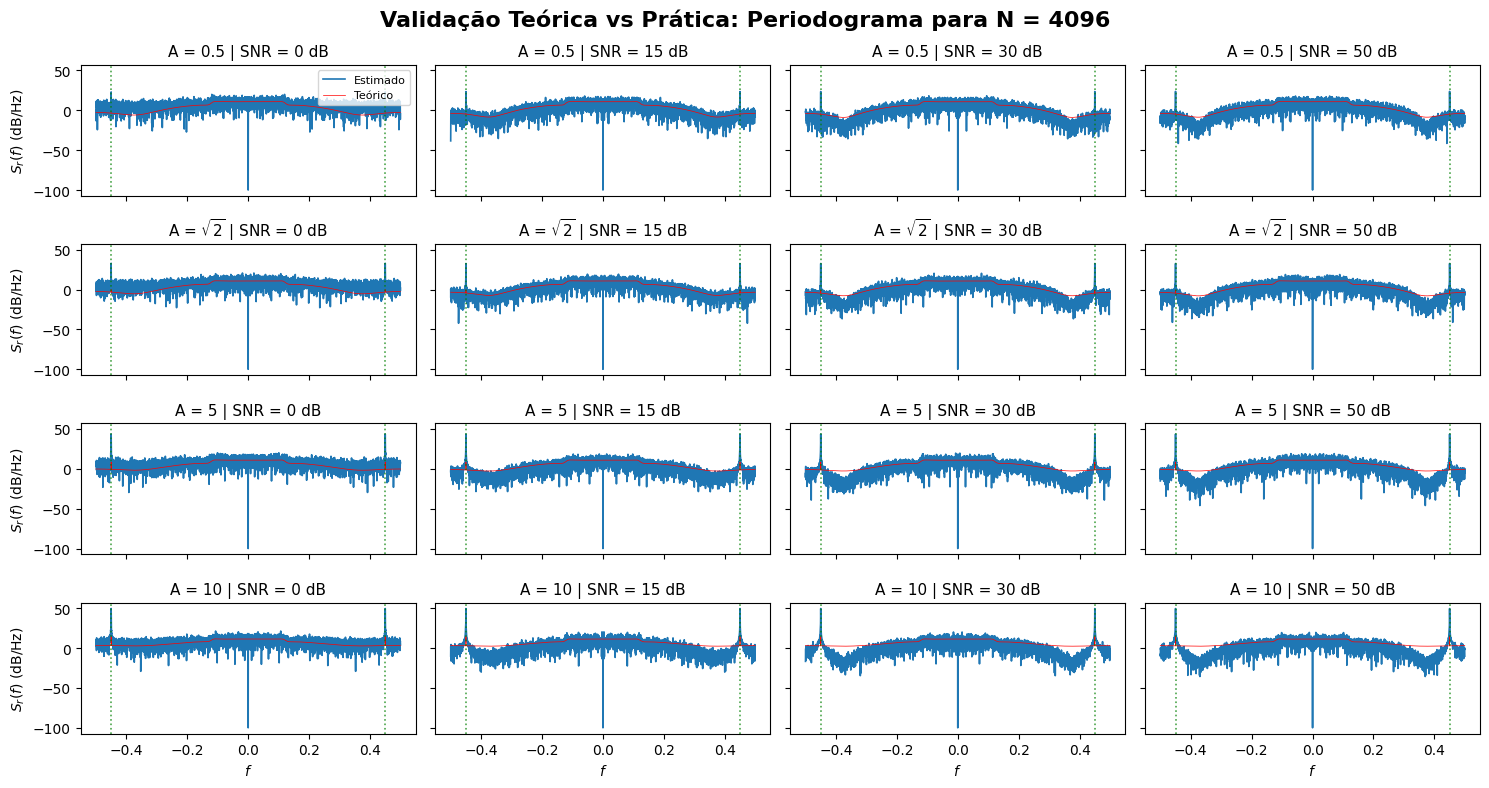
\includegraphics[width=0.9\textwidth]{valid_period_4096.png}
    \end{figure}
\end{frame}

\begin{frame}{Tarefa 4: Resultados de Validação Welch (N=4096)}
    \begin{figure}
        \centering
        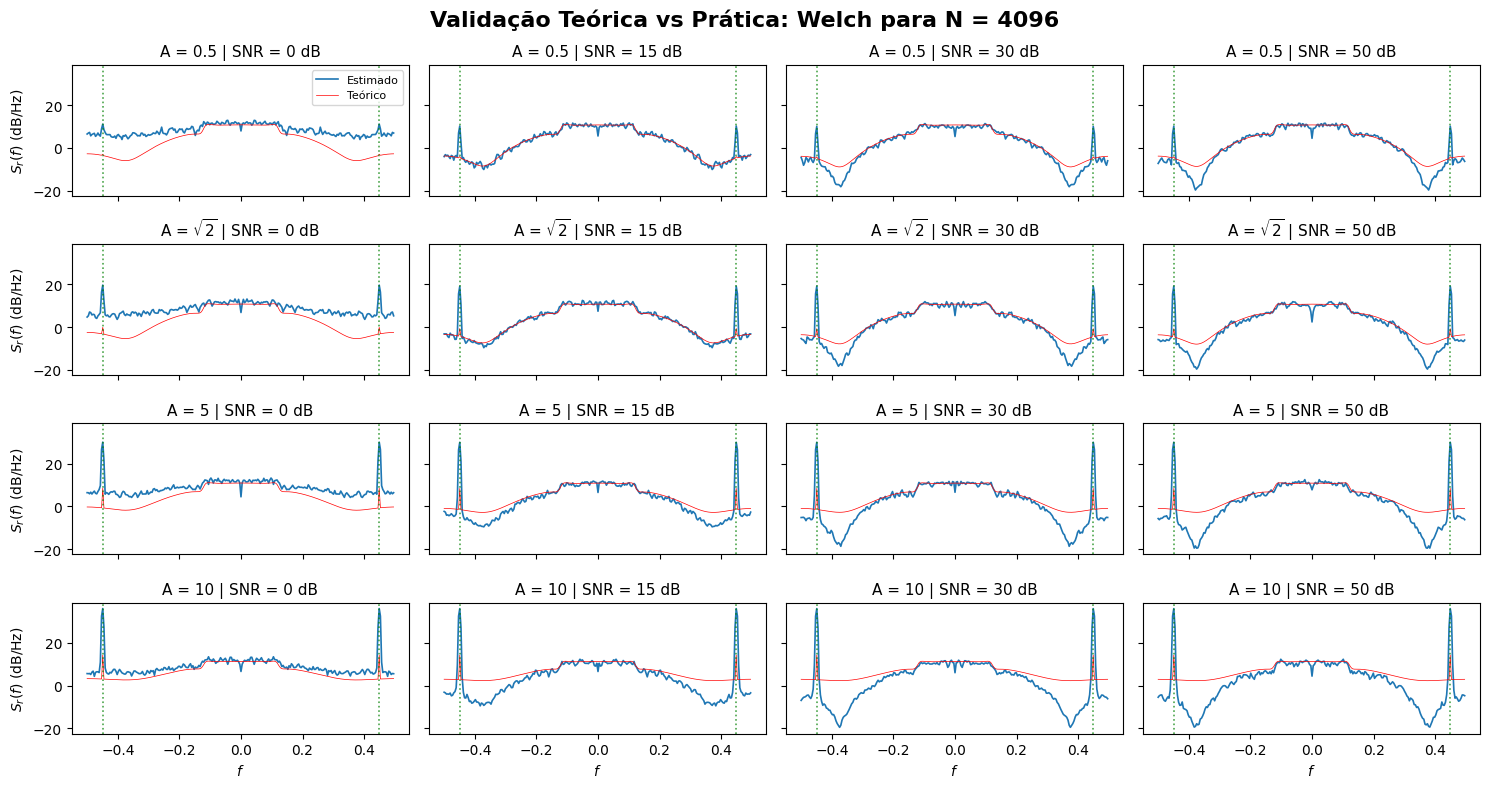
\includegraphics[width=0.9\textwidth]{valid_welch_4086.png}
    \end{figure}
\end{frame}

\begin{frame}{Tarefa 4: Resultados do MSE}
    \begin{itemize}
        \item Menores erros observados para $A=0.5$ e SNR elevadas (15/30 dB).
        \item O Método de Welch tende a apresentar MSE menor em regiões ruidosas devido à suavização.
    \end{itemize}

    \begin{table}
        \centering
        \caption{MSE comparando o teórico com o Welch para N=4096}
        \small % Reduz o tamanho da fonte para caber no slide
        \begin{tabular}{ccc}
            \toprule
            \textbf{A} & \textbf{SNR (dB)} & \textbf{MSE} \\
            \midrule
            0.50  & 0.00  & 15.84 \\
            0.50  & 15.00 & 2.14 \\
            0.50  & 30.00 & 2.26 \\
            0.50  & 50.00 & 2.30 \\
            \midrule
            1.41  & 0.00  & 98.75 \\
            1.41  & 15.00 & 63.86 \\
            1.41  & 30.00 & 64.17 \\
            1.41  & 50.00 & 65.14 \\
            \midrule
            5.00  & 0.00  & 9893.30 \\
            5.00  & 15.00 & 9466.15 \\
            5.00  & 30.00 & 9604.26 \\
            5.00  & 50.00 & 9663.50 \\
            \midrule
            10.00 & 0.00  & 156975.65 \\
            10.00 & 15.00 & 154760.26 \\
            10.00 & 30.00 & 154157.96 \\
            10.00 & 50.00 & 154529.46 \\
            \bottomrule
        \end{tabular}
    \end{table}

\end{frame}

% --- TAREFA 5 ---
\section{Tarefa 5}
\begin{frame}{Tarefa 5: Variando o valor de $L$}
    \begin{itemize}
        \item Variação do tamanho da janela $L \in \{34, 128, 256, 512\}$ para $N=4096$.

        \item Para não gerar um número muito grande de variações (128), foram escolhidos os seguintes
                cenários para análise.
    \end{itemize}

    \vfill

    \begin{block}{Cenários utilizados}
        \begin{center}
            \begin{columns}
                \begin{column}{0.35\textwidth}
                    \textbf{Amplitudes (A):}
                    \begin{itemize}
                        \item $\sqrt{2}$
                        \item $10.0$
                    \end{itemize}
                \end{column}
                \begin{column}{0.35\textwidth}
                    \textbf{SNR (dB):}
                    \begin{itemize}
                        \item $0$ dB
                        \item $15$ dB
                    \end{itemize}
                \end{column}
                
            \end{columns}
        \end{center}
    \end{block}
    

\end{frame}

\begin{frame}{Tarefa 5: Impacto dos diferentes valores de $L$}
    \vfill
    \begin{itemize}
        \item \textbf{L pequeno (34):} Baixa variância, mas apresenta \textit{Spectral Leakage}.
        \item \textbf{L médios (128 / 256):} Acabam por ser a melhor escolha por balancear o melhor dos 2 extremos.
        \item \textbf{L grande (512):} Alta resolução (picos nítidos), porém alta variância (muitas oscilações).
    \end{itemize}
    \vfill
    \begin{block}{Tradeoff bias x variance}
        Janelas maiores melhoram a resolução mas reduzem o número de blocos para média, impedindo a suavização do ruído.
    \end{block}
\end{frame}

\begin{frame}{Tarefa 5: Impacto de L nos Cenários Escolhidos}
    \begin{figure}
        \centering
        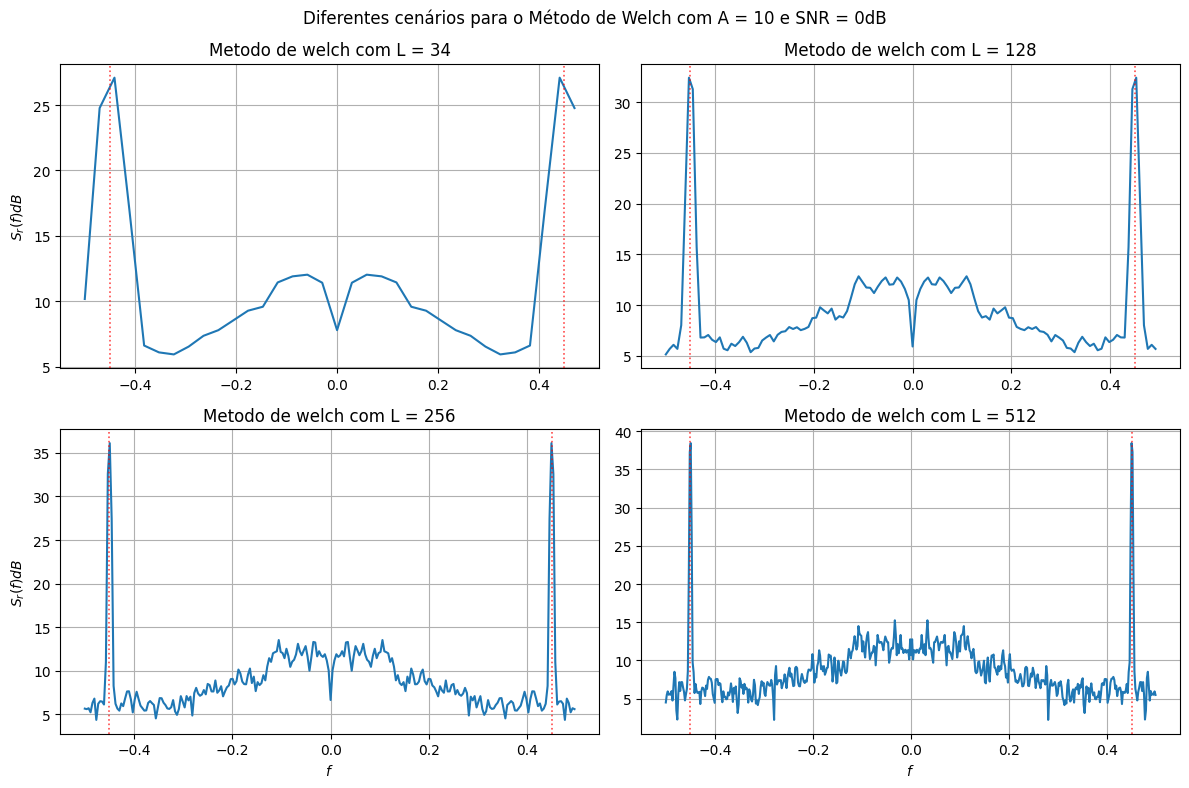
\includegraphics[width=0.8\textwidth]{tarefa5_L_variation_1.png}
    \end{figure}
\end{frame}

\begin{frame}{Tarefa 5: Impacto de L nos Cenários Escolhidos}
    \begin{figure}
        \centering
        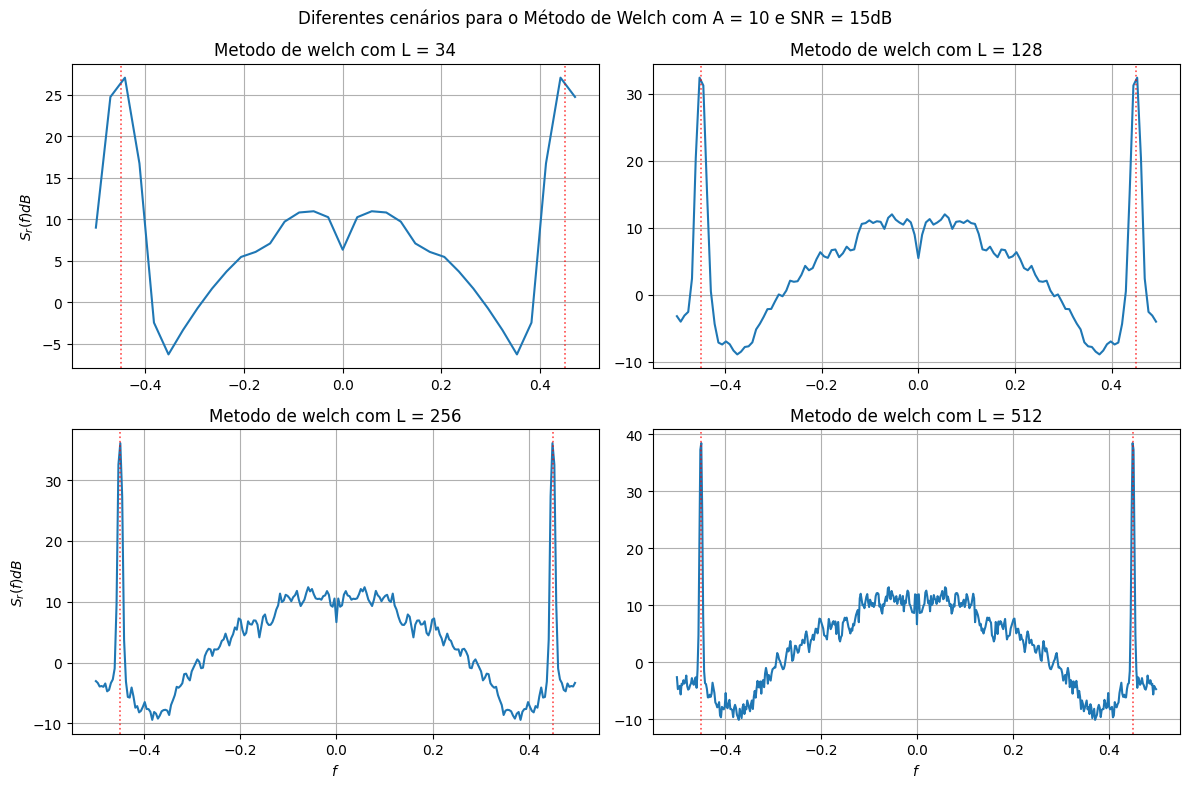
\includegraphics[width=0.8\textwidth]{tarefa5_L_variation_2.png}
    \end{figure}
\end{frame}

\begin{frame}{Tarefa 5: Impacto de L nos Cenários Escolhidos}
    \begin{figure}
        \centering
        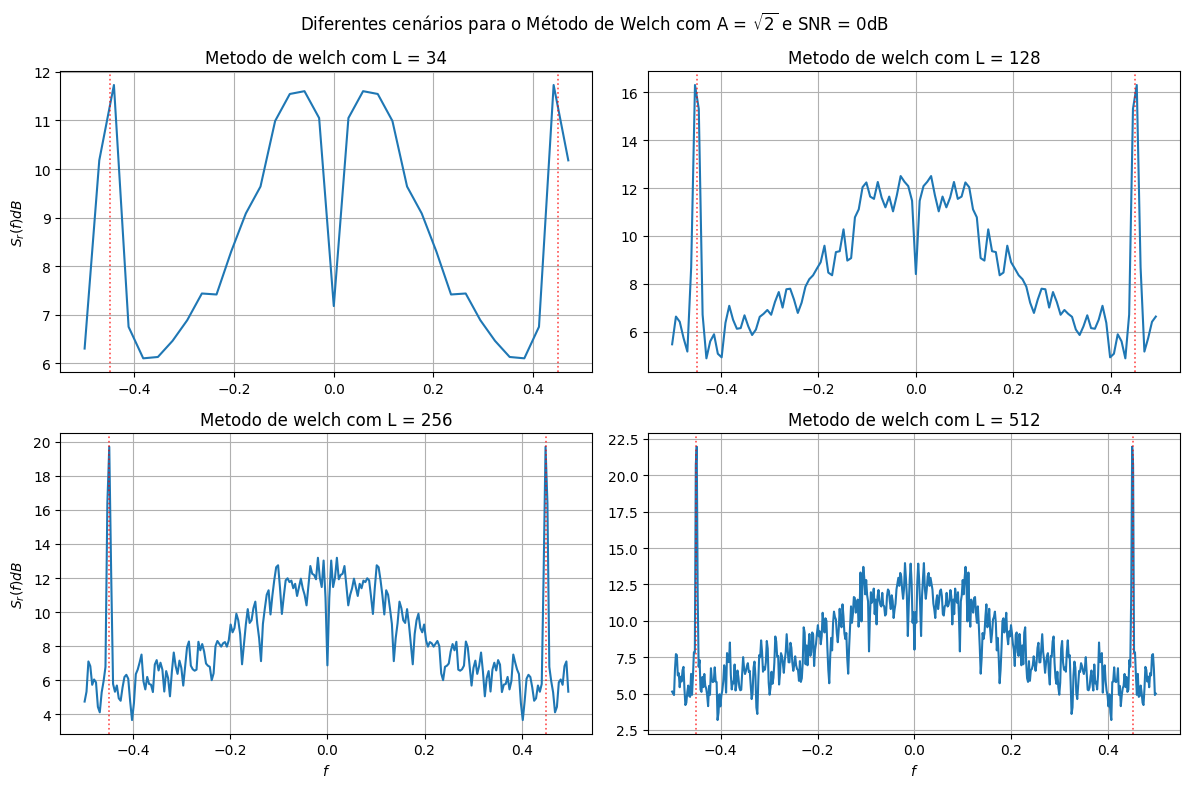
\includegraphics[width=0.8\textwidth]{tarefa5_L_variation_3.png}
    \end{figure}
\end{frame}

\begin{frame}{Tarefa 5: Impacto de L nos Cenários Escolhidos}
    \begin{figure}
        \centering
        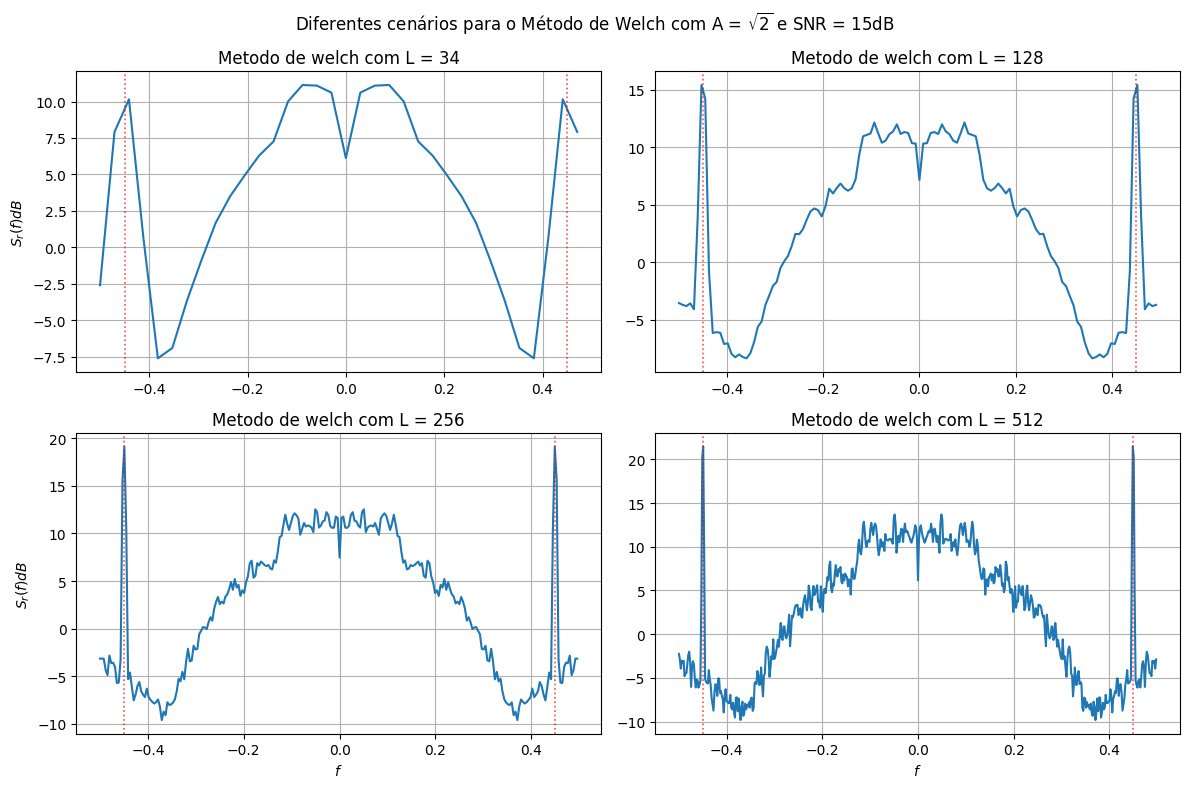
\includegraphics[width=0.8\textwidth]{tarefa5_L_variation_4.png}
    \end{figure}
\end{frame}

\begin{frame}{Tarefa 5: Variância da Estimativa em Função de $L$}
    \vspace{-0.2cm}
    
    % Primeira linha de tabelas (A = 10)
    \begin{columns}[t]
        \begin{column}{0.48\textwidth}
            \centering
            \textbf{A = 10 | SNR = 0 dB} \\ \vspace{0.1cm}
            \scriptsize
            \begin{tabular}{rr}
                \toprule
                \textbf{L} & \textbf{Var} \\
                \midrule
                34 & 17582.80 \\
                128 & 72713.44 \\
                256 & 155444.77 \\
                512 & 299243.44 \\
                \bottomrule
            \end{tabular}
        \end{column}
        
        \begin{column}{0.48\textwidth}
            \centering
            \textbf{A = 10 | SNR = 15 dB} \\ \vspace{0.1cm}
            \scriptsize
            \begin{tabular}{rr}
                \toprule
                \textbf{L} & \textbf{Var} \\
                \midrule
                34 & 17447.87 \\
                128 & 72056.21 \\
                256 & 153629.19 \\
                512 & 296818.55 \\
                \bottomrule
            \end{tabular}
        \end{column}
    \end{columns}

    \vspace{0.4cm} % Espaço entre as linhas
    
    % Segunda linha de tabelas (A = 1.414)
    \begin{columns}[t]
        \begin{column}{0.48\textwidth}
            \centering
            \textbf{A = $\sqrt{2}$ | SNR = 0 dB} \\ \vspace{0.1cm}
            \scriptsize
            \begin{tabular}{rr}
                \toprule
                \textbf{L} & \textbf{Var} \\
                \midrule
                34 & 15.62 \\
                128 & 47.95 \\
                256 & 88.12 \\
                512 & 158.00 \\
                \bottomrule
            \end{tabular}
        \end{column}
        
        \begin{column}{0.48\textwidth}
            \centering
            \textbf{A = $\sqrt{2}$ | SNR = 15 dB} \\ \vspace{0.1cm}
            \scriptsize
            \begin{tabular}{rr}
                \toprule
                \textbf{L} & \textbf{Var} \\
                \midrule
                34 & 21.00 \\
                128 & 47.15 \\
                256 & 81.74 \\
                512 & 141.29 \\
                \bottomrule
            \end{tabular}
        \end{column}
    \end{columns}
\end{frame}
% --- TAREFA 6 ---
\section{Tarefa 6}
\begin{frame}{Tarefa 6: Conclusões sobre os Métodos}
    \begin{block}{Conclusões}
    \begin{itemize}
        \item \textbf{Precisão de $f_0$:} O Método de Welch é superior para
            identificar a frequência de interferência em ambientes ruidosos
            (SNR = 0 dB).
        \item \textbf{Limites de Amplitude:} Para $A < \sqrt{2}$, o sistema
            apresenta dificuldade em isolar a frequência. Conforme $A$ aumenta,
            o pico torna-se evidente ($P \propto A^2$), mas a alta concentração
            de energia potencializa o espalhamento para as bandas vizinhas
            (\textit{Spectral Leakage}).
        \item \textbf{Compromisso de Resolução ($L$):} Janelas curtas ($L =
            34$) agravam estruturalmente o \textit{Spectral Leakage}, enquanto
            janelas longas ($L = 512$) disparam a variância da estimativa.
            Portanto, resoluções intermediárias (128 a 256) entregam o balanço
            ideal entre precisão espectral e estabilidade visual.
    \end{itemize}
    \end{block}
\end{frame}

% --- TAREFA 7 ---
\section{Tarefa 7: Estimação de SNR por Sub-bandas}

\begin{frame}{Tarefa 7: Metodologia de Estimação}
    A SNR estimada é calculada isolando e comparando a energia em diferentes regiões do espectro:
    
    \begin{equation*}
        SNR_{\text{est}} = 10 \log_{10} \left( \frac{P_{\text{SinalPuro}}}{P_{\text{RuídoTotal}}} \right)
    \end{equation*}
    
    \vspace{0.3cm}
    \textbf{Intervalos de Frequência Adotados:}
    \begin{itemize}
        \item \textbf{Zona do Sinal} $[ -0.20, 0.20 ]$
        \item \textbf{Zona Neutra de Ruído} $[ 0.25, 0.40 ]$
    \end{itemize}
\end{frame}

\begin{frame}{Tarefa 7: Tabela de Resultados}
    \begin{table}
        \centering
        \caption{Resultados da Estimação de SNR}
        \scriptsize % Fonte reduzida para caber no slide
        \begin{tabular}{cccc}
            \toprule
            \textbf{Amplitude (A)} & \textbf{SNR Teórica} & \textbf{L} & \textbf{SNR Estimada (dB)} \\
            \midrule
            
            % Bloco A = 10, SNR = 0
            10.000 & 0 dB  & 34  & -1.99 \\
                   &       & 128 & -1.36 \\
                   &       & 256 & -1.33 \\
                   &       & 512 & -1.39 \\
            \midrule
            
            % Bloco A = 10, SNR = 15
            10.000 & 15 dB & 34  & 6.27 \\
                   &       & 128 & 7.10 \\
                   &       & 256 & 7.18 \\
                   &       & 512 & 7.35 \\
            \midrule
            
            % Bloco A = 1.414, SNR = 0
            $\sqrt{2}$  & 0 dB  & 34  & -1.53 \\
                   &       & 128 & -1.38 \\
                   &       & 256 & -1.24 \\
                   &       & 512 & -1.35 \\
            \midrule
            
            % Bloco A = 1.414, SNR = 15
            $\sqrt{2}$  & 15 dB & 34  & 7.52 \\
                   &       & 128 & 7.94 \\
                   &       & 256 & 7.93 \\
                   &       & 512 & 8.20 \\
            \bottomrule
    \end{tabular}
    \end{table}
\end{frame}

\begin{frame}{Tarefa 7: Conclusões da Estimação}
    A análise dos dados revela que a eficácia depende do nível do ruído AWGN do sistema:
    
    \begin{itemize}
        \item \textbf{Robustez em Ambientes Ruidosos ($0\text{ dB}$):} Como o
            ruído de fundo tem alta energia e se distribui uniformemente por
            toda a banda, a medição na Zona Neutra é precisa. O estimador
            entrega valores coerentes (próximos a $-1.3\text{ dB}$).
        \item \textbf{Saturação em Ambientes com Menos Ruído ($15\text{ dB}$):} A 
            estimação travou em um limite superior com valor $\in (7, 8)$
            dB na maioria dos casos, tanto para interferências fortes ($A$ =
            10) quanto mais fracas ($A$ = $\sqrt{2}$).
        \item \textbf{Possivel Causa:} Com o ruído em níveis muito baixos, a
            energia da que vaza para a zona neutra (\textit{Spectral Leakage})
            passa a ser contabilizada incorretamente.
    \end{itemize}
\end{frame}

% --- Slide Final ---
\begin{frame}
    \centering
    \Huge Obrigado! \\
    \vfill
    \Large Dúvidas?
\end{frame}

\end{document}
